\chapter{Point Cloud Visibility}
\label{ch:visibility}
This chapter introduces our custom point cloud visibility algorithm. It starts by giving in Section~\ref{sc:spec-visibility}, a clear context for the presented work. Then, Section~\ref{sc:related-visibility} gives an overview of the previous related work and describes some experimentations of a previously-published point cloud visibility algorithm. Finally, as nothing seems to be well adjusted for our specific case we implemented a custom point cloud visibility algorithm described in Section~\ref{sc:custom}.

\section{Specifications}
\label{sc:spec-visibility}

\subsection{Context}
Currently in \CC, there is a way to still use a point cloud for reconstructing purposes even if the scanner's location information is lost. It gives the user the opportunity to manually set the scanners position on a 3D representation of the point cloud. But, only one position can be set. It requires that the point cloud contains points resulting from \emph{one and only one} scanner\footnote{Also known as monoscan point cloud.}. This is because, during the reconstruction, \CC uses
the scanner location to orient the normals at each point. In a monoscan point cloud case, it simply orients each normal toward the scanner. But in case of multiscan point cloud, it needs to know for each point, toward which scanner the normal must be oriented, which is difficult to find.

Therefore, even if \emph{ScanFinder} (Chapter~\ref{ch:scanfinder}) is applied on a LAS format\footnote{A point cloud format that \CC wants to support and which does not store scanner locations in its metadata.} multiscan point cloud in order to retrieve all scanner positions, the reconstruction is still infeasible for \CC. This is where a point cloud visibility algorithm is useful in order to attribute each point to a scanner. Have in mind that a point can be seen by two scanners, especially if there is no physical barrier between them. In this case it is difficult to exactly know which scanner produced the point. But, as this point-scanner attribution is only required for normal orientations, we only need to know which scanner best sees it.

\subsection{Objective}
\label{subsc:vis-objective}
As a final step toward supporting point clouds without scanner locations, the algorithm must:
\begin{itemize}
\item take as input any 3D point cloud captured from static scanners as well as the location of all scanners,
\item be invariant to differences between scanners, such as: density, noise, rotation angle,
\item find for each point the scanner which best sees it, not necessary the scanner which produced it,
\item have a reasonnable running time.
\end{itemize}

As for \emph{ScanFinder} described in Chapter~\ref{ch:scanfinder}, the algorithm is not expected to work with mobile point clouds.


\section{Related work}
\label{sc:related-visibility}
This section highlight some previous work on the subject of \emph{Point cloud visibility} before describing in detail one approach that we tried and the obtained results.

\subsection{Previous work}
Visibility in point clouds is a topic that experienced several publications since the 1960s~\cite{appel, sutherland, funkhouser, greene, bittner}. Some methods solve this problem in a 3D rendering context by estimating normals and reconstructing surfaces \cite{sainz1, sainz2, wald, wu}. This contrasts with our case as we need visible points in order to reconstruct surfaces. Another common approach is to use z-buffering techniques based on point depths~\cite{dachsbacher} to reconstruct
surfaces in a real-time rendering context. Even if this approach can be adapted to compute visibility of all points from all scanner location viewpoints, it is not robust to noisy point clouds.

One elegant approach compute point cloud visibility without surface reconstruction: \cite{vis1}. This approach is invariant to point cloud density and only point coordinates are needed (no normal estimation). It uses simple operations: an inversion followed by a convex hull computation. However, it is not robust enough againt LiDAR point cloud noises. An improved version \cite{vis2} has been implemented, see Section~\ref{subsc:noisy}. Although it brings concavity robustness, the same observation is made; it is not robust enough against LiDAR point cloud noise. In both papers, only small\footnote{Compare to LiDAR point clouds.} and enclosed surfaces are reconstructed. They seems to not be fitted for LiDAR point clouds.

In Section~\ref{sc:custom} we describe a custom point cloud visibility algorithm suited for our needs (Section~\ref{subsc:vis-objective}). It is robust to point cloud noise, avoid point occlusions and assigh each point to a scanner.

\subsection{An interesting approach: Visibility of Noisy Point Cloud Data}
\label{subsc:noisy}
As previously said, the \emph{Visibility of Noisy Point Cloud Data}~\cite{vis1} paper describes some improvements of \emph{Direct visibility of point sets}~\cite{vis1} for a better handling of noise and concave surfaces in point clouds. This section summerizes both papers.

\subsubsection{Overview}
The purpose of \cite{vis1} is to discard directly from the point cloud, which point is \emph{hidden}. The problem being solved is: Given a set of points $P$ (considered a sampling of continuous surface $S$) and a viewpoint $C$, determine the points in $P$ visible from $C$. They introduced the HPR (Hidden Point Removal) Operator. This operator uses two simple operations:
\begin{itemize}
  \item an inversion
  \item a convex hull computation
\end{itemize}

\begin{figure}[h]
  \centering
  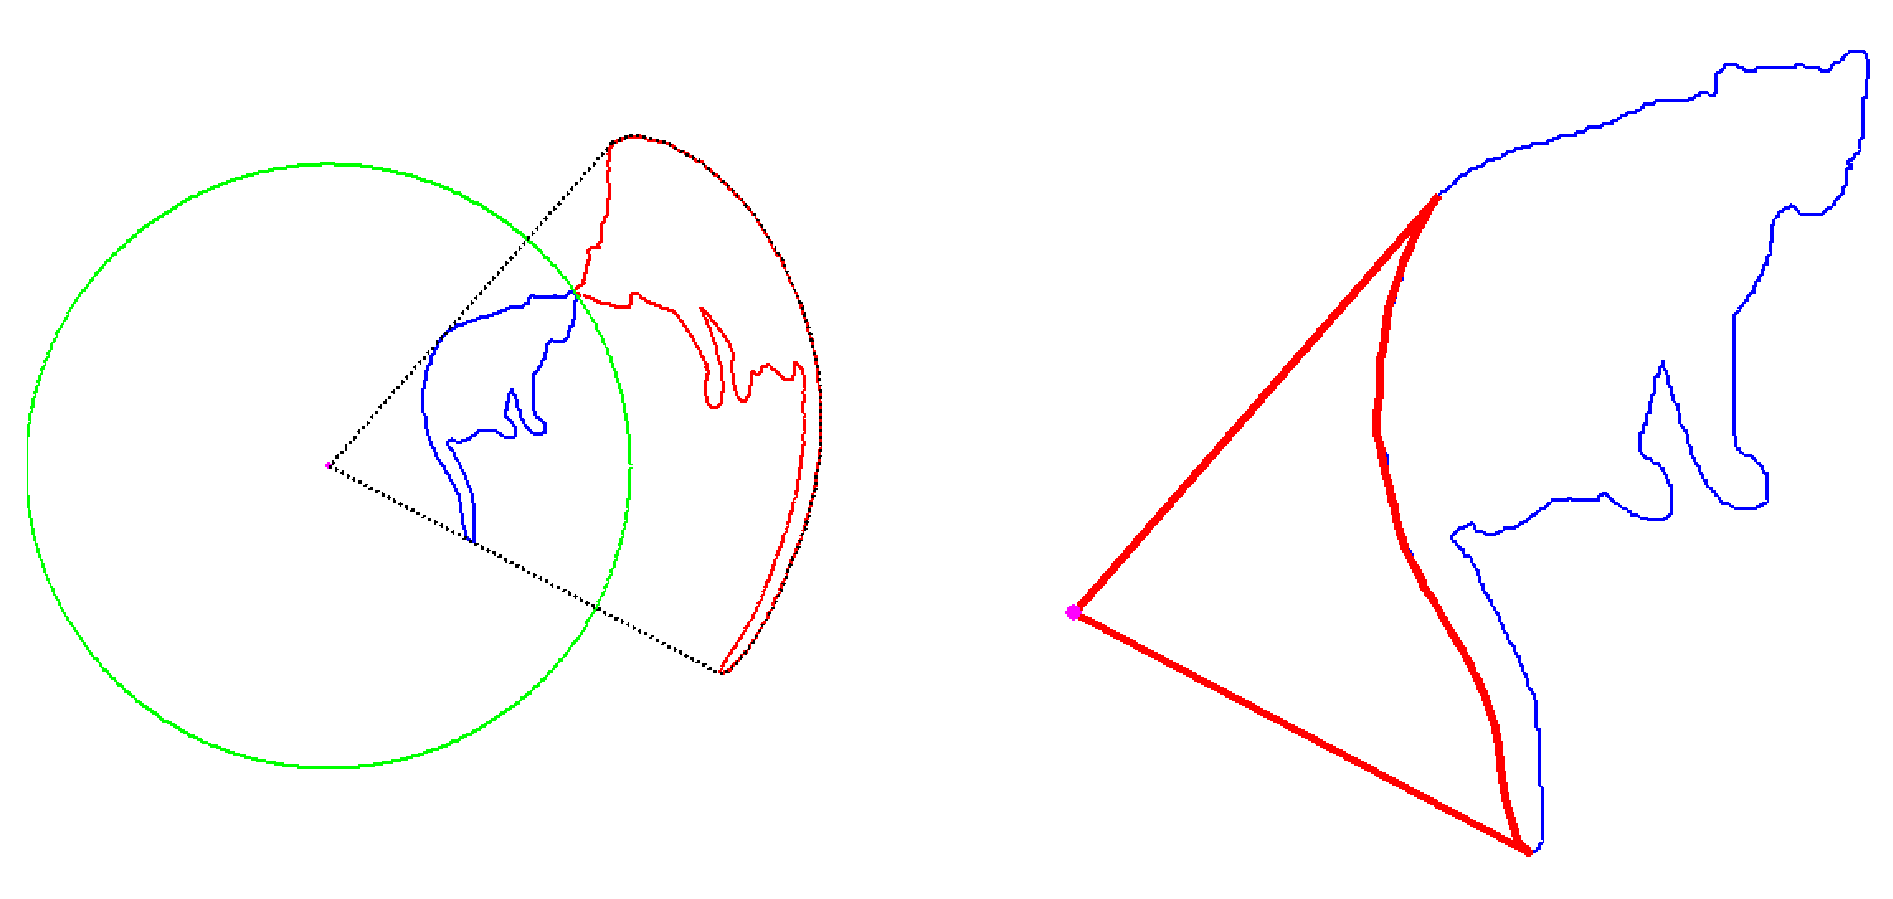
\includegraphics[scale=0.2]{img/hpr.png}
  \caption{HPR operator: on the left a spherical flipping (in red) of a curve (in blue) using a sphere (in green), on the right: a back projection of the convex hull.}
  \label{fig:hpr}
\end{figure}
\begin{figure}[h]
  \centering
  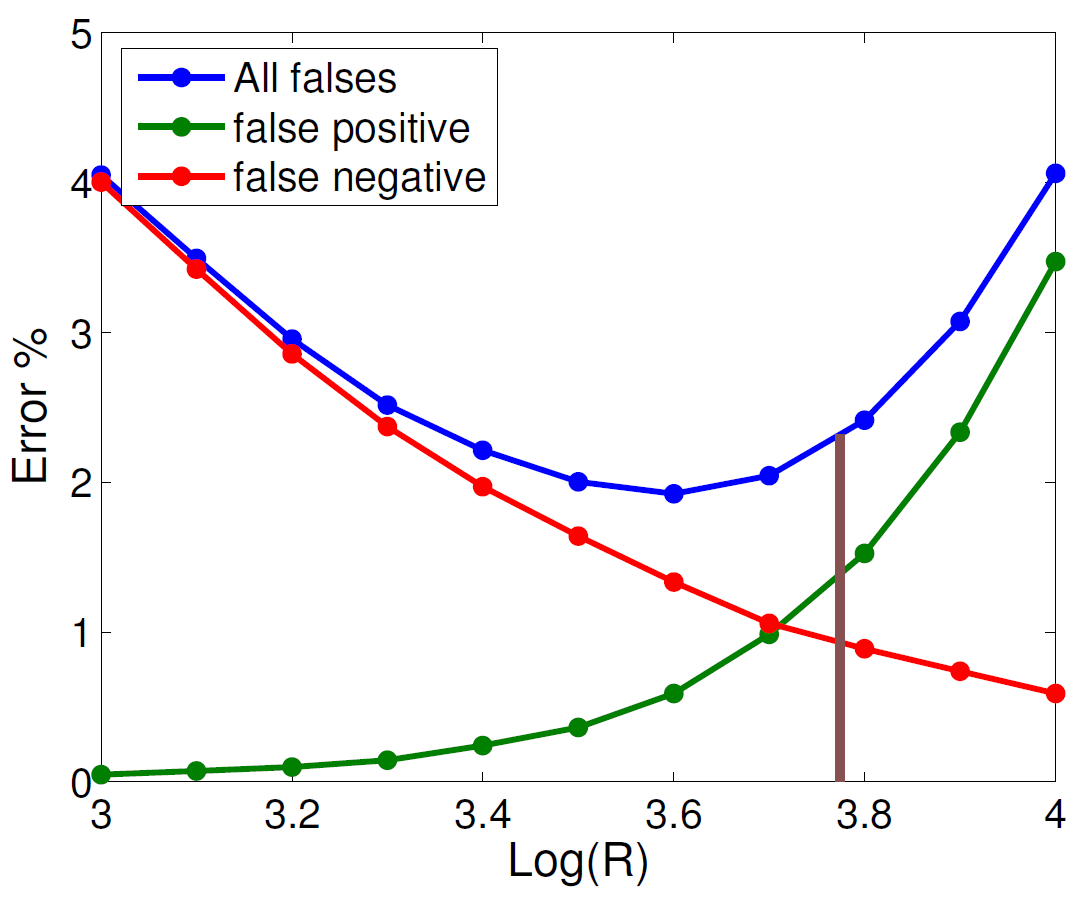
\includegraphics[scale=0.35]{img/hpr-r.png}
  \caption{The variation of, in one hand the spherical inversion ray $R$ and in the other, the percentage of visibility detection error.}
  \label{fig:hpr-r}
\end{figure}

Figure~\ref{fig:hpr} shows both operation results. On the left is performed a spherical flipping (the inversion) of the point cloud, centered at the viewpoint $C$. In this example, the ray $R$ of the sphere seems to be $R_\text{max}$: \emph{the distance from $C$ to the furthest point}. However, the HPR authors suggest to use a second viewpoint (the opposite of the current viewpoint) and vary $R$ while maximizing the number of points considered visible by a unique viewpoint. Figure~\ref{fig:hpr-r} shows on the same plot, for a particular point cloud, the estimated $R=R_\text{opt}$ (in brown) and the percentage or error of the method while varying $R$.\\
A spherical inversion based on the depth of the points put the nearest points (must of them visible) further away. The second step on the right, based on a convex hull computation, detects visible points. A point lying on this convex hull is considered as visible. Even if a visible point is far in the real domain and closer in the inverted domain it should be on this convex hull, as long as it is visible -- no points behind it, no points hidding it.

Although this method is simple, has only meaningful computations and an interesting complexity $\mathcal{O}(n\log{}n)$, it is not robust enough against noisy point clouds, in particular LiDAR ones. With a small $R$, visible points may be marked as non-visible by HPR. On the contrary, with a large $R$, non-visible points may be considered as visible. Moreover, this method handles poorly concave forms; it requirs a low curvature in case of concavity.

These concerns have been addressed in the \emph{Visibility of Noisy Point Cloud Data} paper~\cite{vis2}. They conducted some experiences leading to:
\begin{itemize}
  \item a boundary on the $R$ value that must be respected:
    \begin{equation*}
      ma_{\text{max}} \leq R \leq \left( \frac{\alpha D}{2 \sigma} + 1 \right) \left( \frac{a_{\text{min}} - \sigma}{4} \right)
    \end{equation*}
  \item a guard band on the convex hull which helps to consider as visible all points closer than $2 \times \epsilon_{\text{max}}$ to the convex hull.
    \begin{equation*}
      \epsilon_\text{max} = \left( \frac{4R}{a_\text{min} - \sigma} - 1 \right) \sigma
    \end{equation*}
  \item an iterative method for concavity robustness. It varies $R$ value within the range. For each $R$ value it computes points visibility and update points weight based on the number of times they are tagged as visible. The idea is that high curvatures becore visible at higher values while others (convex, oblique, planar) are consistently visible. The is the function $f$ used in the Algorithm~\ref{alg:RobustHPR}..
\end{itemize}

\begin{figure}[h]
  \centering
  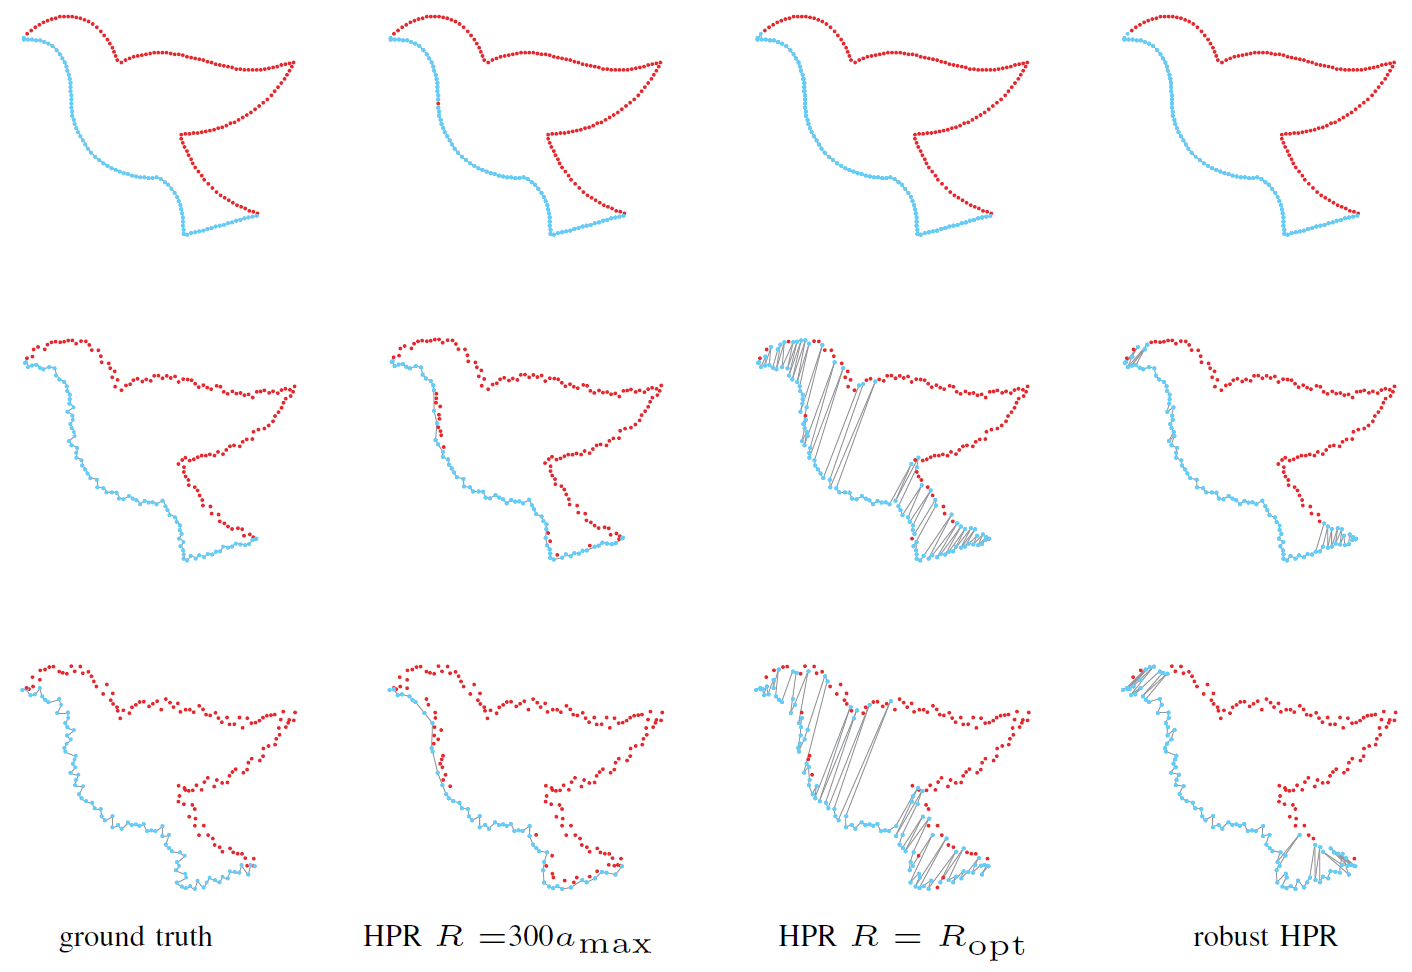
\includegraphics[scale=0.35]{img/rhpr-result.png}
  \caption{Result comparing HP$R_\text{max}$, HP$R_\text{opt}$ and Robust HPR}
  \label{fig:rhpr-result}
\end{figure}

Figure~\ref{fig:rhpr-result} shows some results comparing this method (Robust HPR) with the original methods, one using $R = R_\text{max}$ and the other $R = R_\text{opt}$. It may be observed that Robust HPR achieves better results than the others. The algorithm is shown below (Algorithm~\ref{alg:RobustHPR}). Note that here, the way $R$ is computed is the content of the function $f$.

\begin{algorithm}[tb]
  \SetAlgoVlined
  \DontPrintSemicolon
  \SetKw{Report}{report}
  \SetArgSty{}
  \SetKwFunction{RobustHPR}{RobustHPR}
  \SetKwProg{Fn}{Function}{:}{}
  \Fn{\RobustHPR{$P$, $C$}}{
    \KwIn{
      \begin{itemize}
        \item a set of points $P = \left\lbrace p_i \mid i \in [0, s]  \right\rbrace$,
        \item the viewpoint $C$.
      \end{itemize}
    }
    \KwOut{a the set $V$ of visible points}
    \;
    $P' \gets \emptyset$ \tcp{contains inverted points}
    $\Delta' \gets \emptyset$ \tcp{contains inverted hidden points}
    $R \gets f(P, C)$\tcp{Compute the spherical inversion ray $R$}
    \;
    \tcp{spherical inversion}
    \ForEach{$p_i \in P$}{
      $P' \gets P' \cup \left\lbrace p_i' = p_i + 2 \left( R - \left\lVert p_i  \right\rVert  \right) \frac{p_i}{\left\lVert p_i \right\rVert} \right\rbrace$
    }
    \;
    \tcp{compute the convex hull of $P' \cup \left\lbrace C \right\rbrace$ in order to put aside visible points}
    $\Delta' \gets \text{convex\_hull}(P' \cup \left\lbrace C \right\rbrace)$\;
    \;
    \tcp{Catch all points within a $2 \times \epsilon_\text{max}$ distance form the convex hull points}
    $\epsilon_\text{max} \gets \left( \frac{4R}{a_\text{min} - \sigma} - 1 \right) \sigma$\;
    \ForEach{$p_i' \in \Delta'$}{
      \ForEach{$p_j' \in \Delta'$ belonging to the $50$ nearest points of $p_i'$}{
        \If{$\left\lVert p_i' - p_j' \right\rVert \leq 2\epsilon_\text{max}$}{
          $\Delta' \gets \Delta' \cup \left\lbrace p_j' \right\rbrace$\;
        }
      }
    }
    \;
    \tcp{Back projection of hidden points}
    $\Delta \gets \left\lbrace p_i \in P \mid p_i' \in \Delta' \right\rbrace$\;
    \;
    \Return{$ P \setminus \Delta $}\;
  }
  \caption{The robust HPR algorithm.\label{alg:RobustHPR}}
\end{algorithm}




\subsubsection{Results and discussions}


\section{A custom disk-based approach}
\label{sc:custom}

\subsection{Overview}


\subsection{Implementation}


\subsection{Results and discussions}
